\begin{figure}[H]
    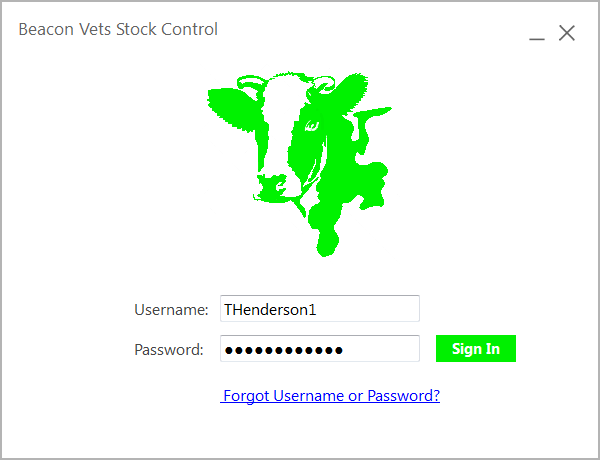
\includegraphics[width=\textwidth]{./101-1.png}
    \caption{Entering Valid Log In Details At The Log In Screen} \label{fig:101-1}
\end{figure}

\begin{figure}[H]
    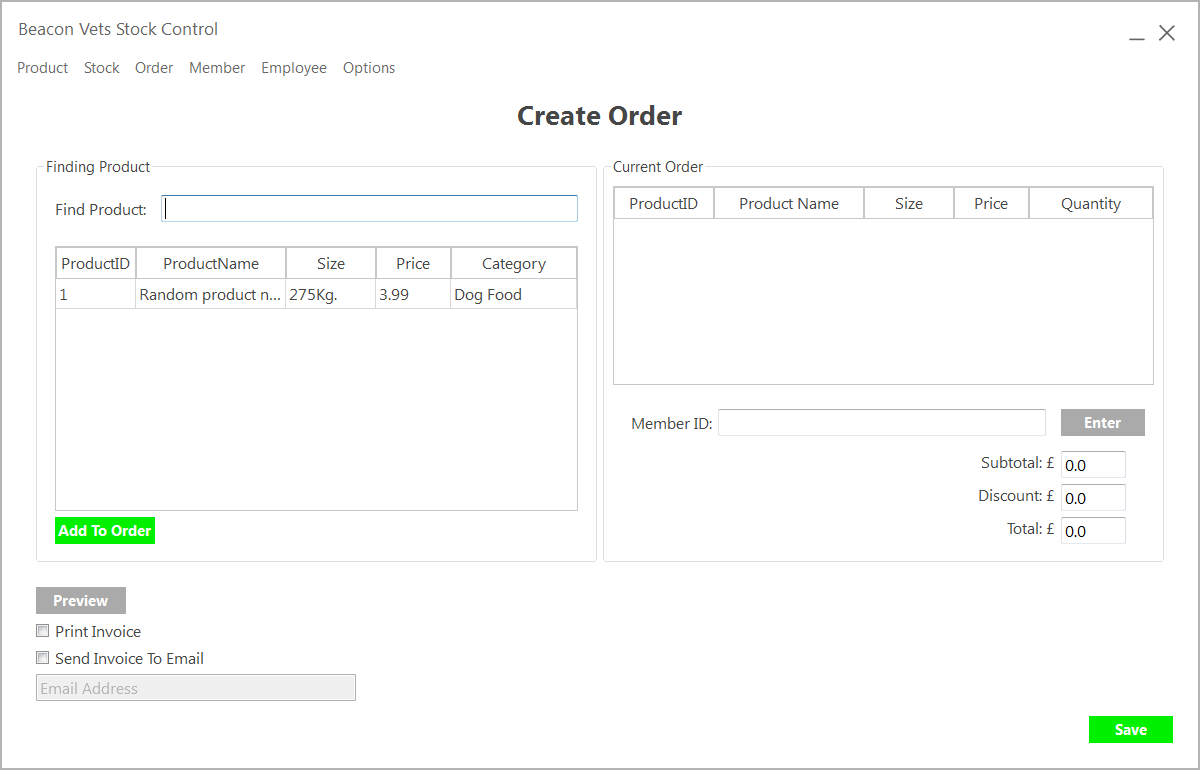
\includegraphics[width=\textwidth]{./101-2.png}
    \caption{Clicking Log In Button with Valid Details} \label{fig:101-2}
\end{figure}

\begin{figure}[H]
    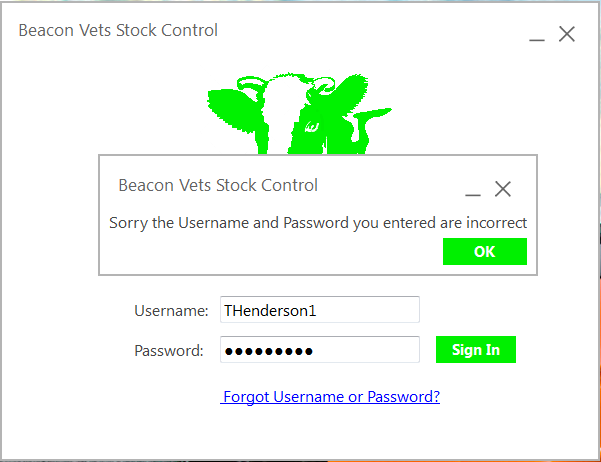
\includegraphics[width=\textwidth]{./101-3.png}
    \caption{Trying to sign in with invalid details} \label{fig:101-3}
\end{figure}

\begin{figure}[H]
    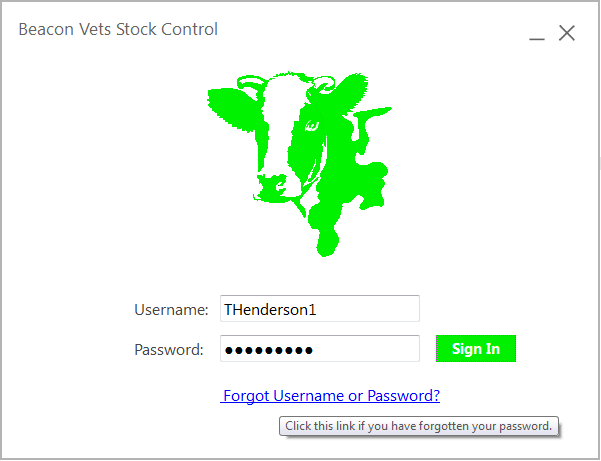
\includegraphics[width=\textwidth]{./102-1.png}
    \caption{Clicking Forgot Username or Password Button} \label{fig:102-1}
\end{figure}

\begin{figure}[H]
    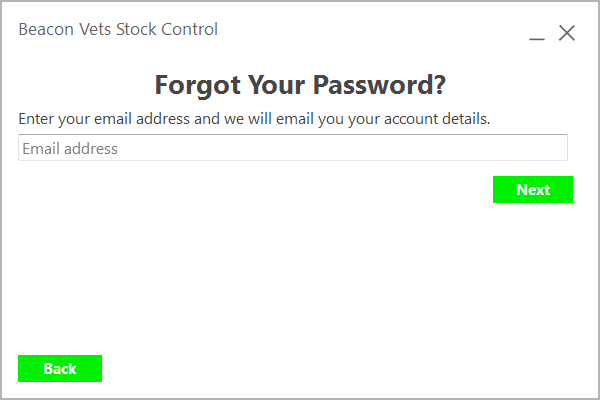
\includegraphics[width=\textwidth]{./102-2.png}
    \caption{After Clicking on the Forgot Password Button } \label{fig:102-2}
\end{figure}

\begin{figure}[H]
    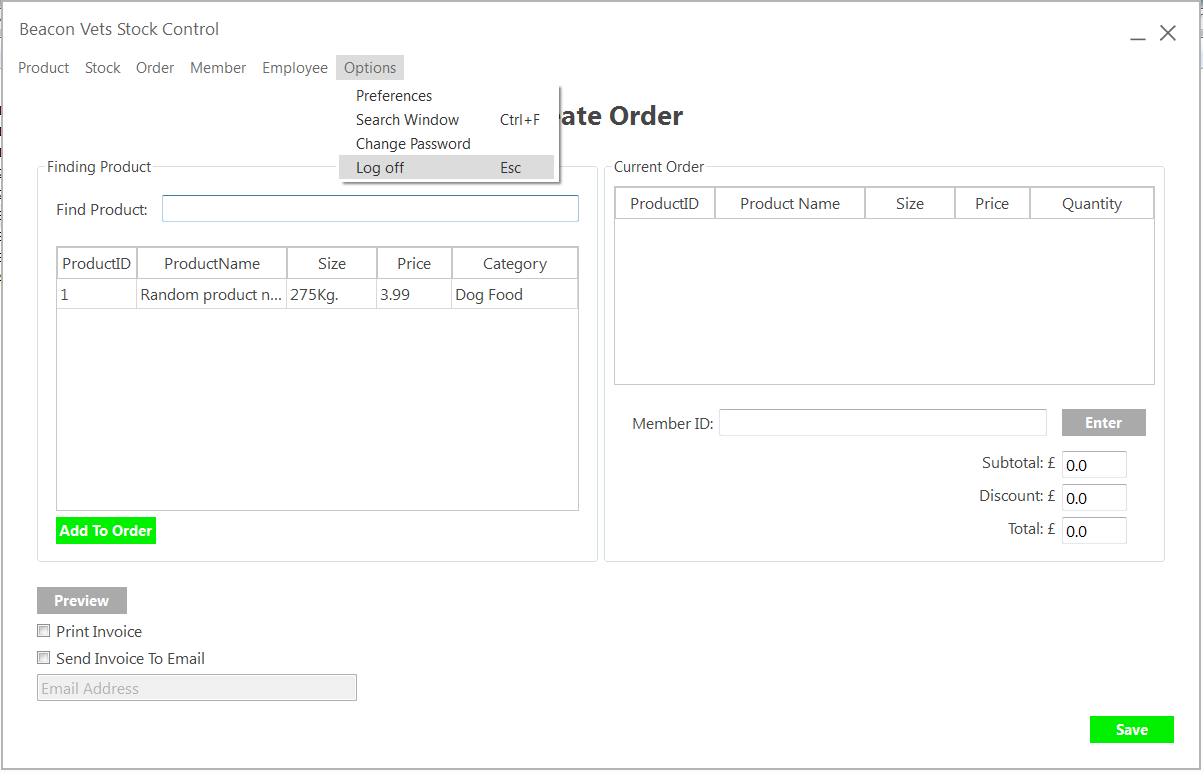
\includegraphics[width=\textwidth]{./103-1.png}
    \caption{Clicking The Log Off button} \label{fig:103-1}
\end{figure}

\begin{figure}[H]
    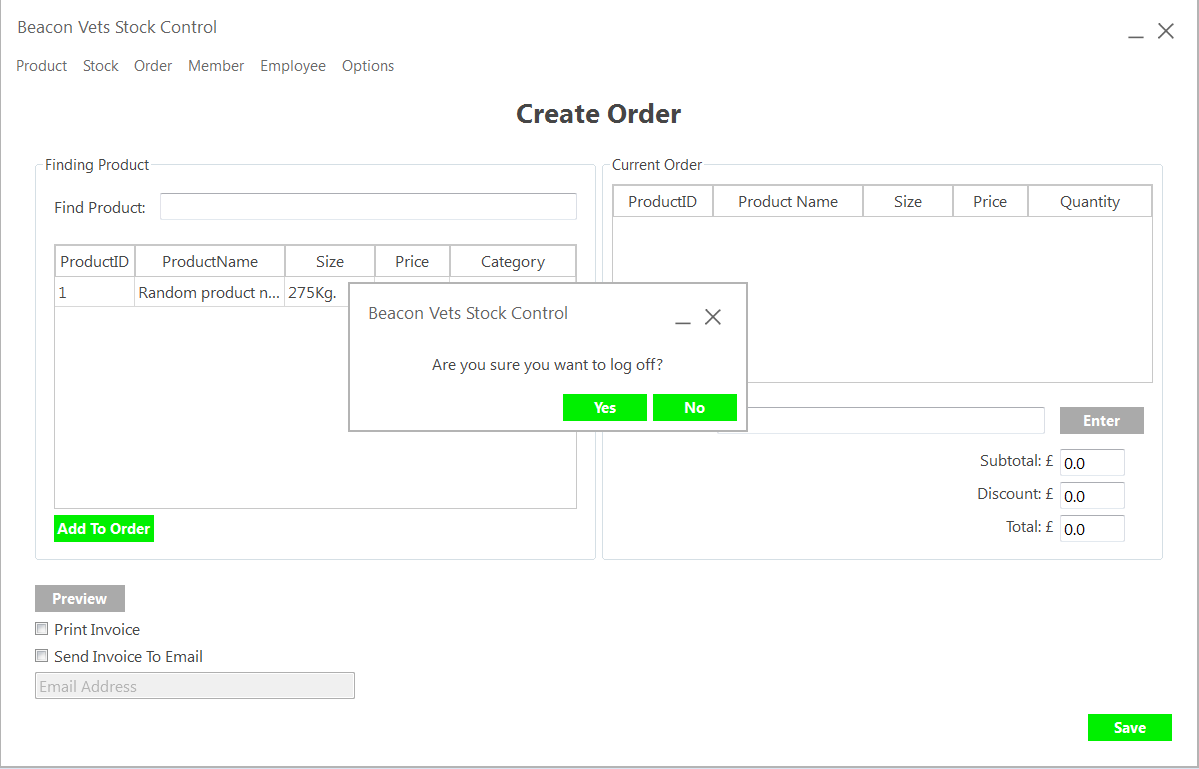
\includegraphics[width=\textwidth]{./103-2.png}
    \caption{Log Off Confirmation Window} \label{fig:103-2}
\end{figure}

\begin{figure}[H]
    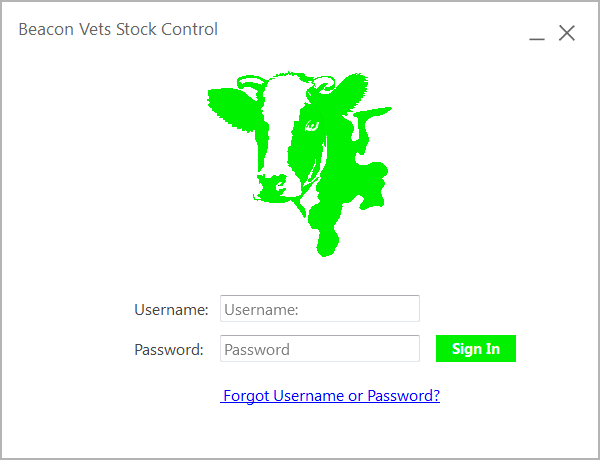
\includegraphics[width=\textwidth]{./103-3.png}
    \caption{After Clicking Yes on the Log Off Decision} \label{fig:103-3}
\end{figure}

\begin{figure}[H]
    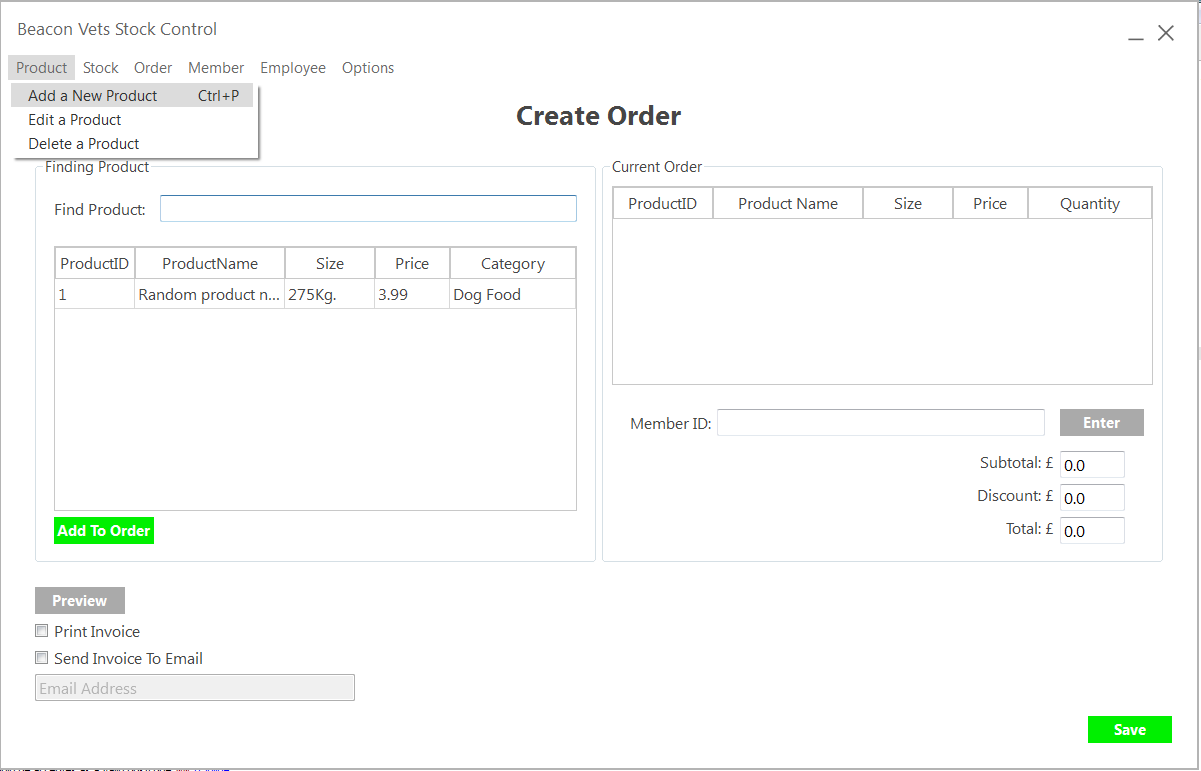
\includegraphics[width=\textwidth]{./104-1.png}
    \caption{Clicking The Add Product Button Under The Product Menu} \label{fig:104-1}
\end{figure}

\begin{figure}[H]
    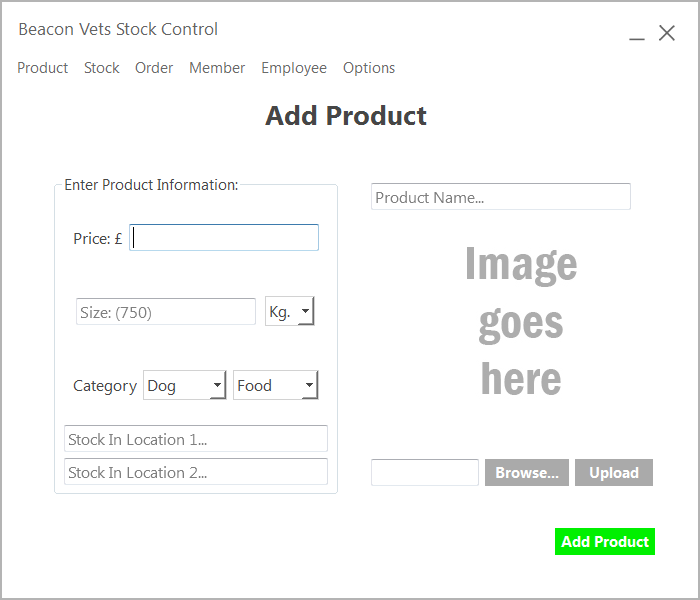
\includegraphics[width=\textwidth]{./104-2.png}
    \caption{The Add Product Interface} \label{fig:104-2}
\end{figure}

\begin{figure}[H]
    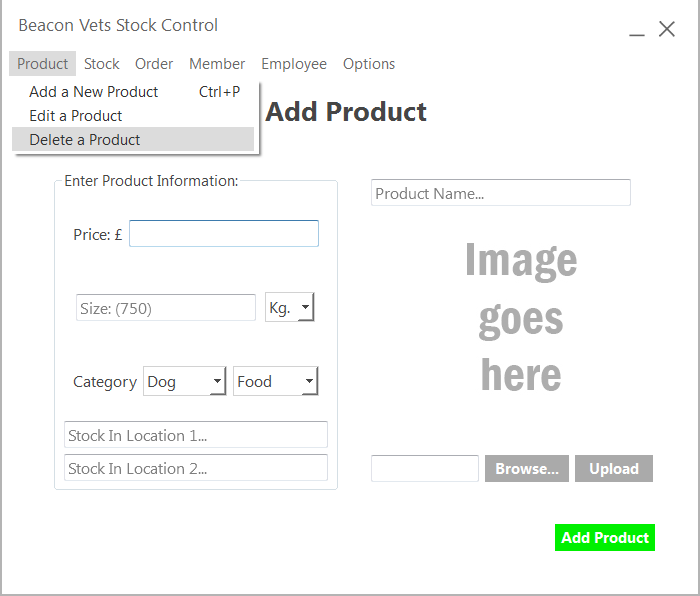
\includegraphics[width=\textwidth]{./105-1.png}
    \caption{Clicking the Delete Product Button Under the Product Menu} \label{fig:105-1}
\end{figure}

\begin{figure}[H]
    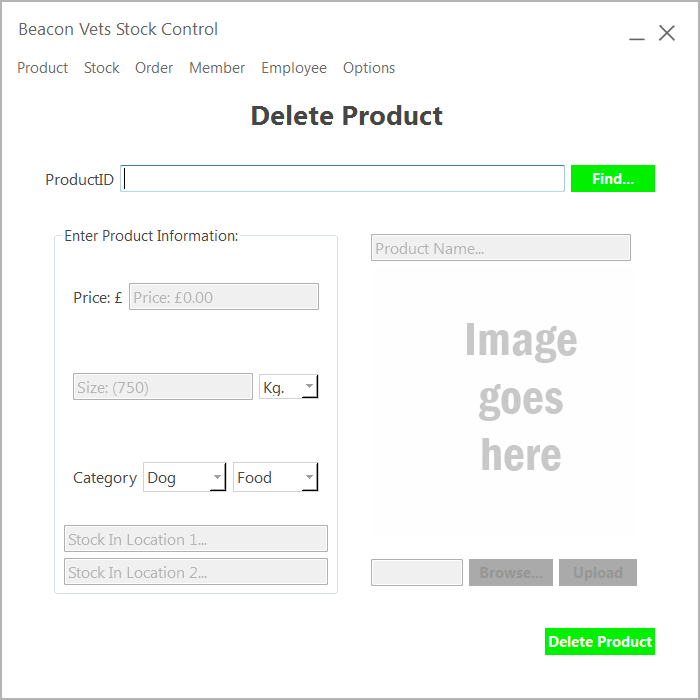
\includegraphics[width=\textwidth]{./105-2.png}
    \caption{Delete Product Interface} \label{fig:105-2}
\end{figure}

\begin{figure}[H]
    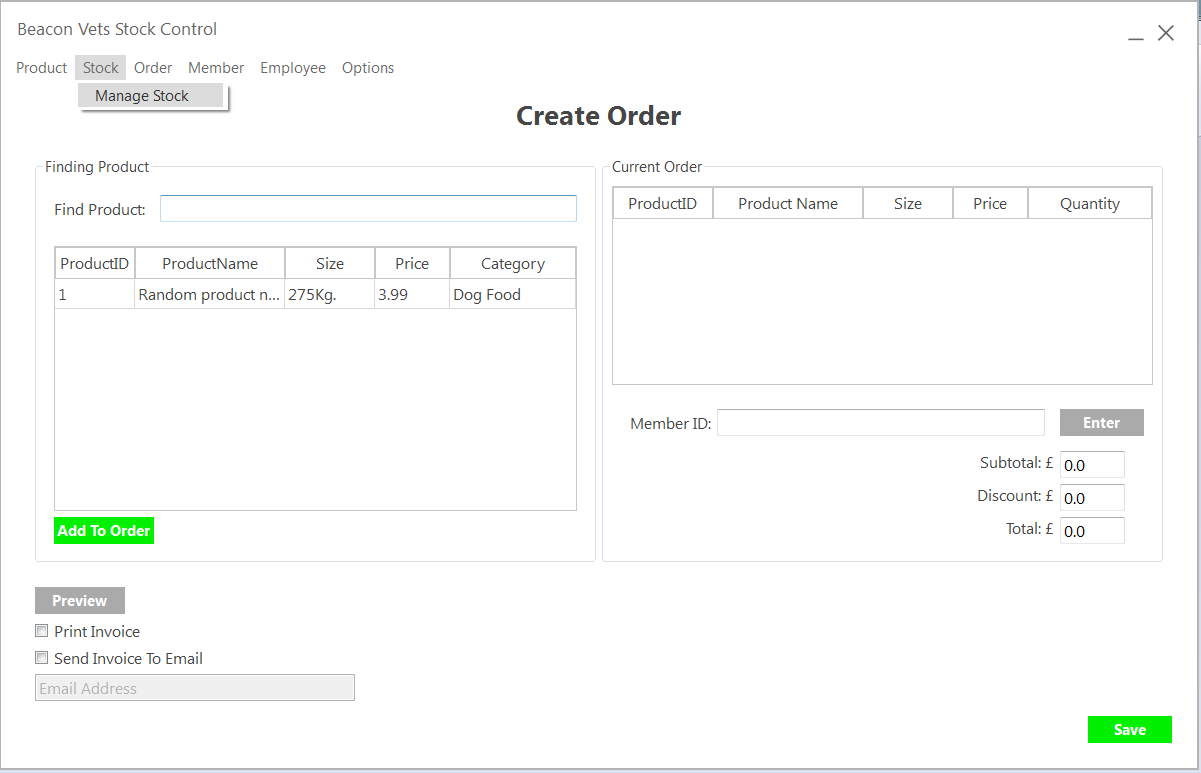
\includegraphics[width=\textwidth]{./106-1.png}
    \caption{Clicking the Manage Stock Button Under the Stock Menu.} \label{fig:106-1}
\end{figure}

\begin{figure}[H]
    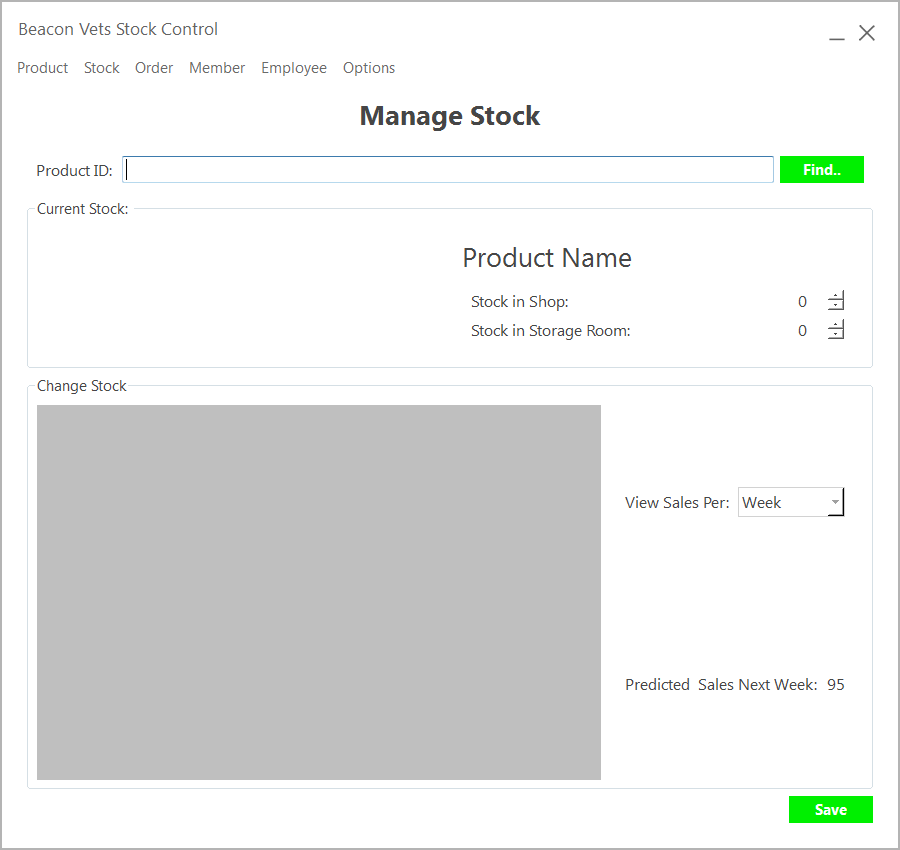
\includegraphics[width=\textwidth]{./106-2.png}
    \caption{Manage Stock Interface} \label{fig:106-2}
\end{figure}

\begin{figure}[H]
    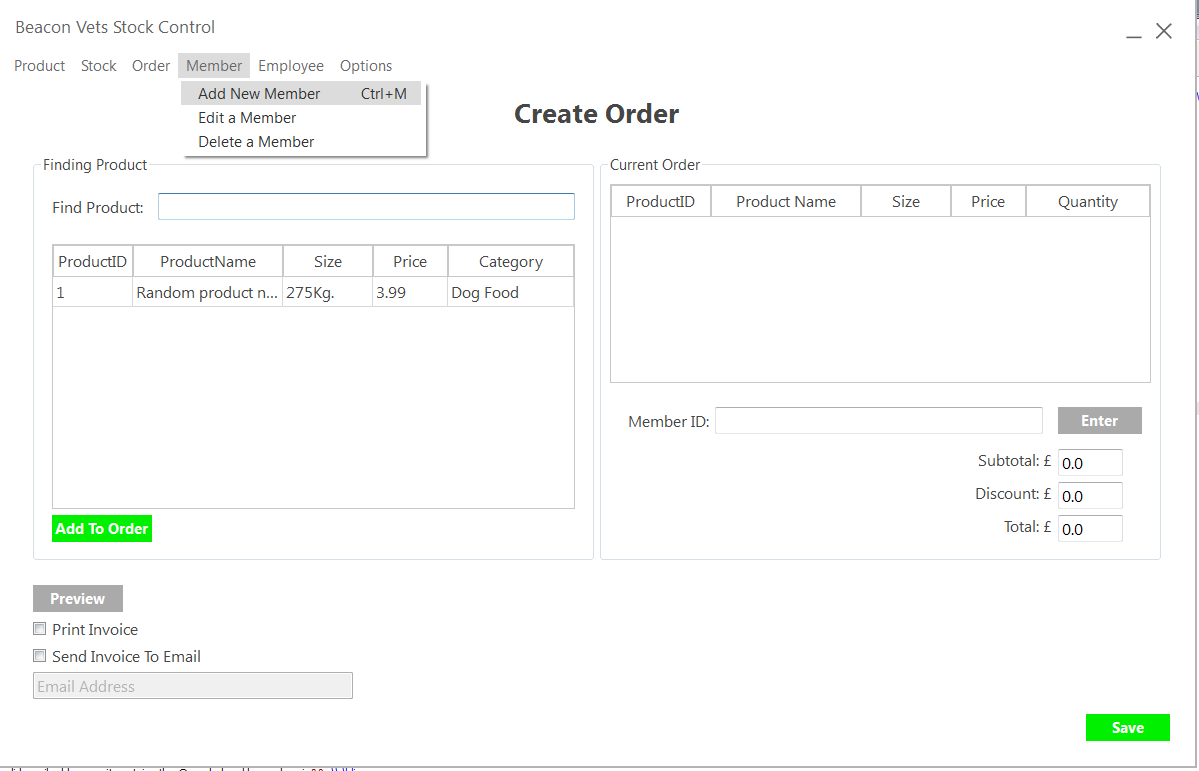
\includegraphics[width=\textwidth]{./107-1.png}
    \caption{Clicking the Adding Member Interface} \label{fig:107-1}
\end{figure}

\begin{figure}[H]
    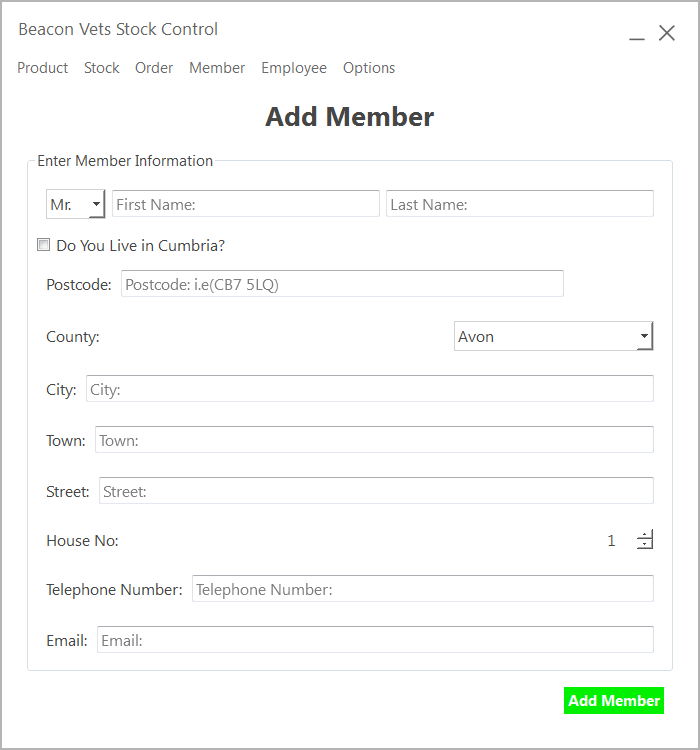
\includegraphics[width=\textwidth]{./107-2.png}
    \caption{Adding Member Interface} \label{fig:107-2}
\end{figure}

\begin{figure}[H]
    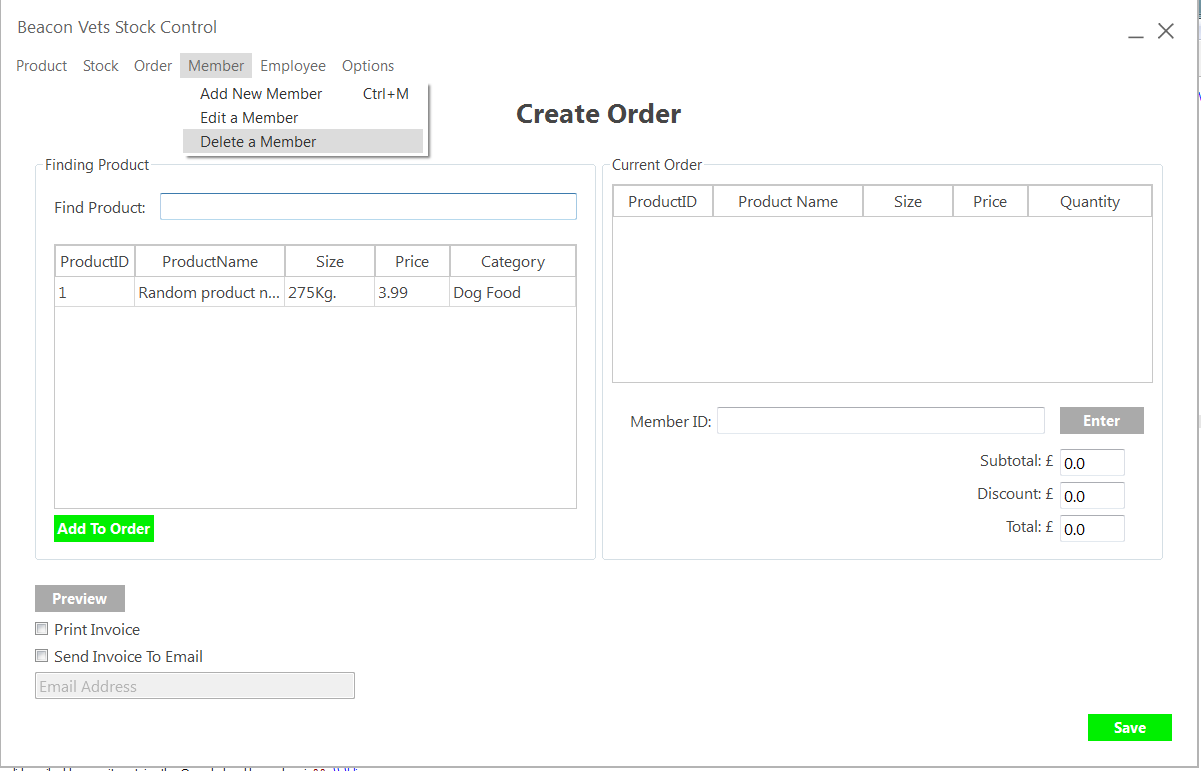
\includegraphics[width=\textwidth]{./108-1.png}
    \caption{Clicking the Delete Member Option Under the Member Menu} \label{fig:108-1}
\end{figure}

\begin{figure}[H]
    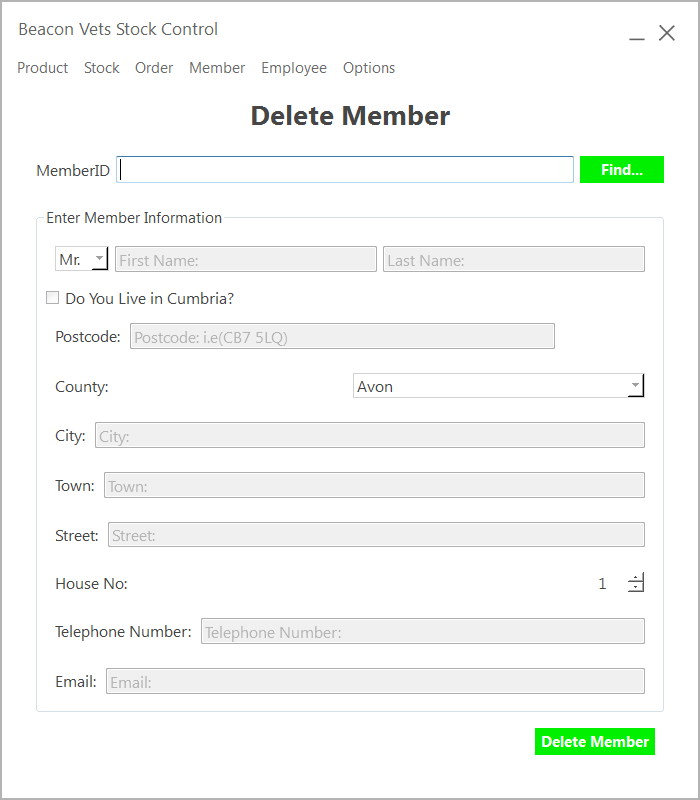
\includegraphics[width=\textwidth]{./108-2.png}
    \caption{The Delete Member Interface} \label{fig:108-2}
\end{figure}

\begin{figure}[H]
    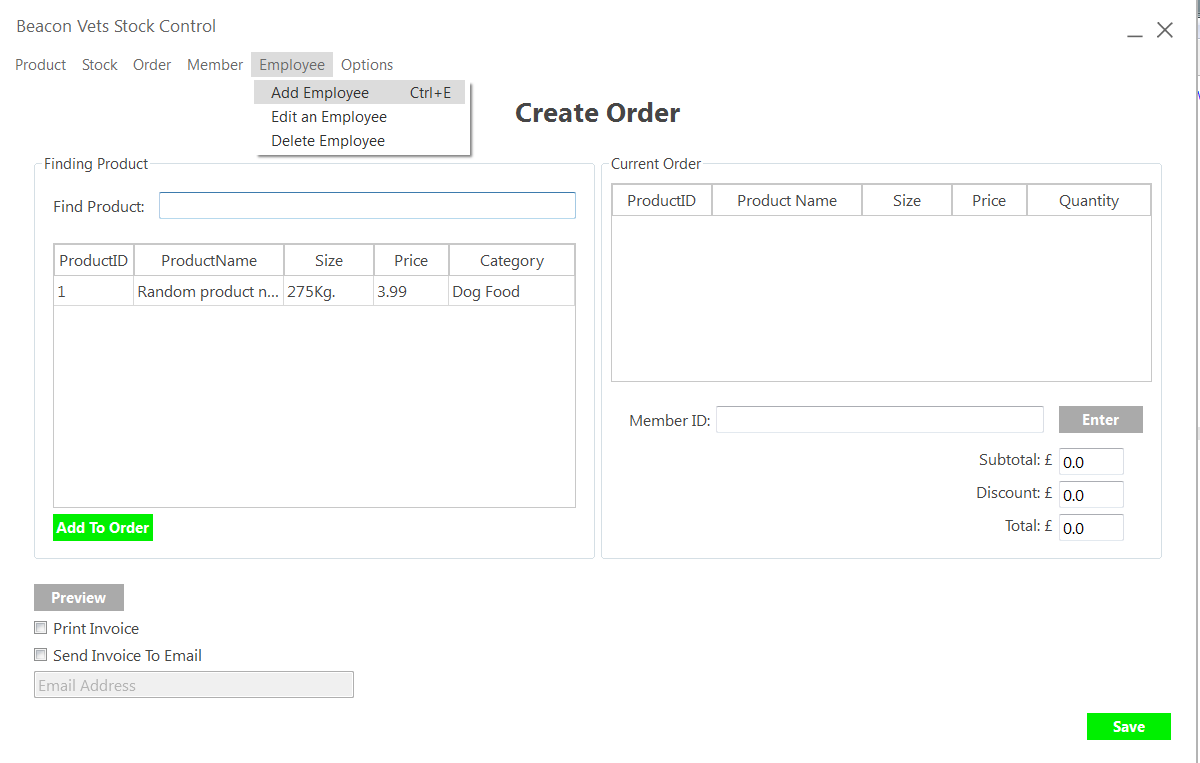
\includegraphics[width=\textwidth]{./109-1.png}
    \caption{Clicking Add Employee Button under Employee Menu} \label{fig:109-1}
\end{figure}

\begin{figure}[H]
    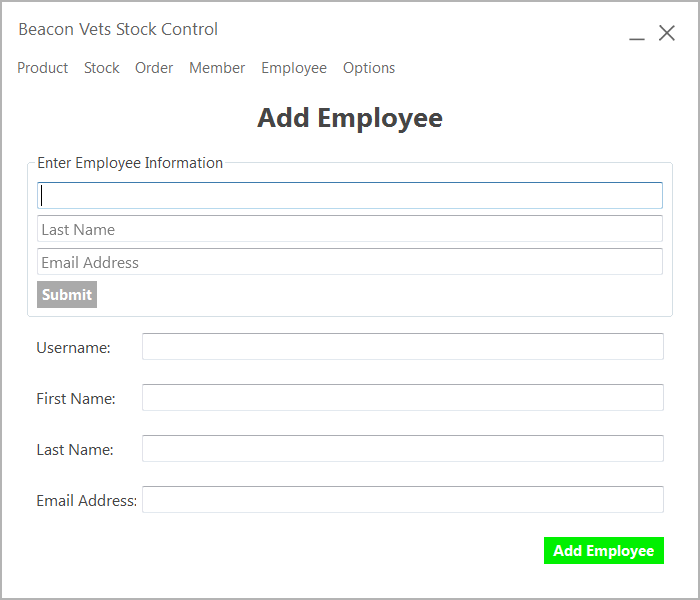
\includegraphics[width=\textwidth]{./109-2.png}
    \caption{The Add Employee Interface} \label{fig:109-2}
\end{figure}

\begin{figure}[H]
    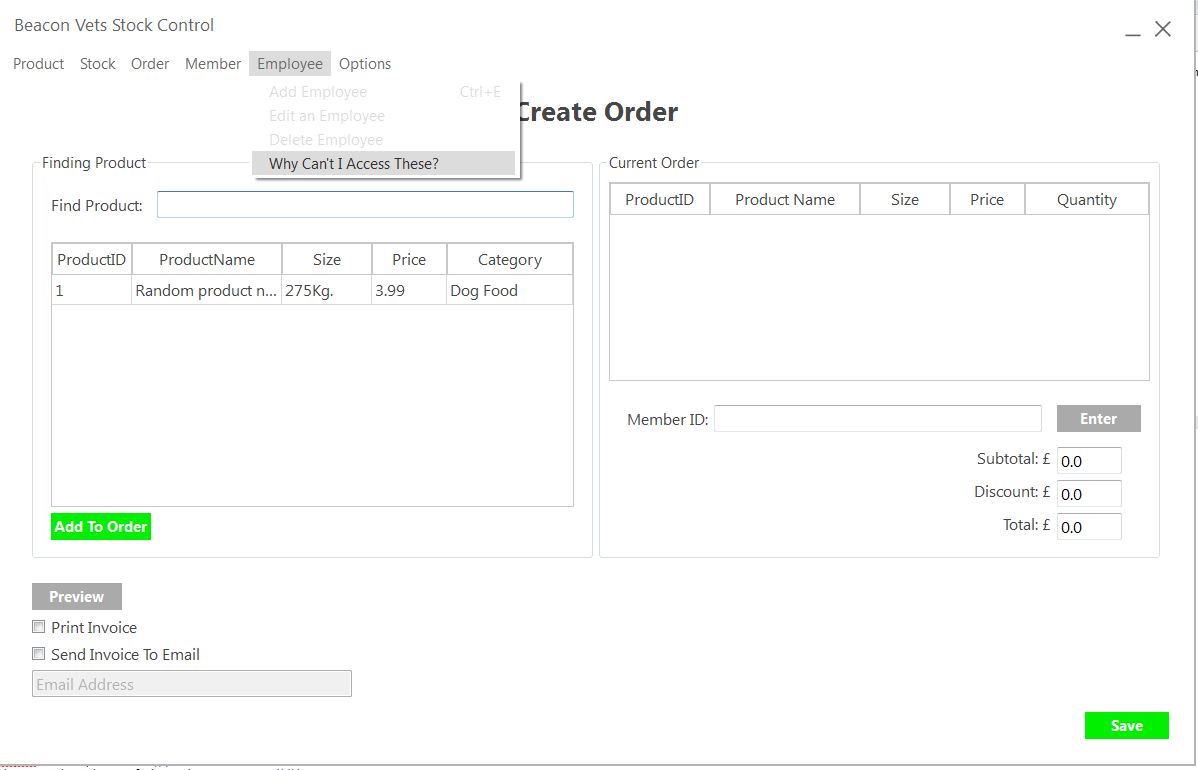
\includegraphics[width=\textwidth]{./109-3.png}
    \caption{Menu that is displayed When not Logged in on the Administrator Account} \label{fig:109-3}
\end{figure}

\begin{figure}[H]
    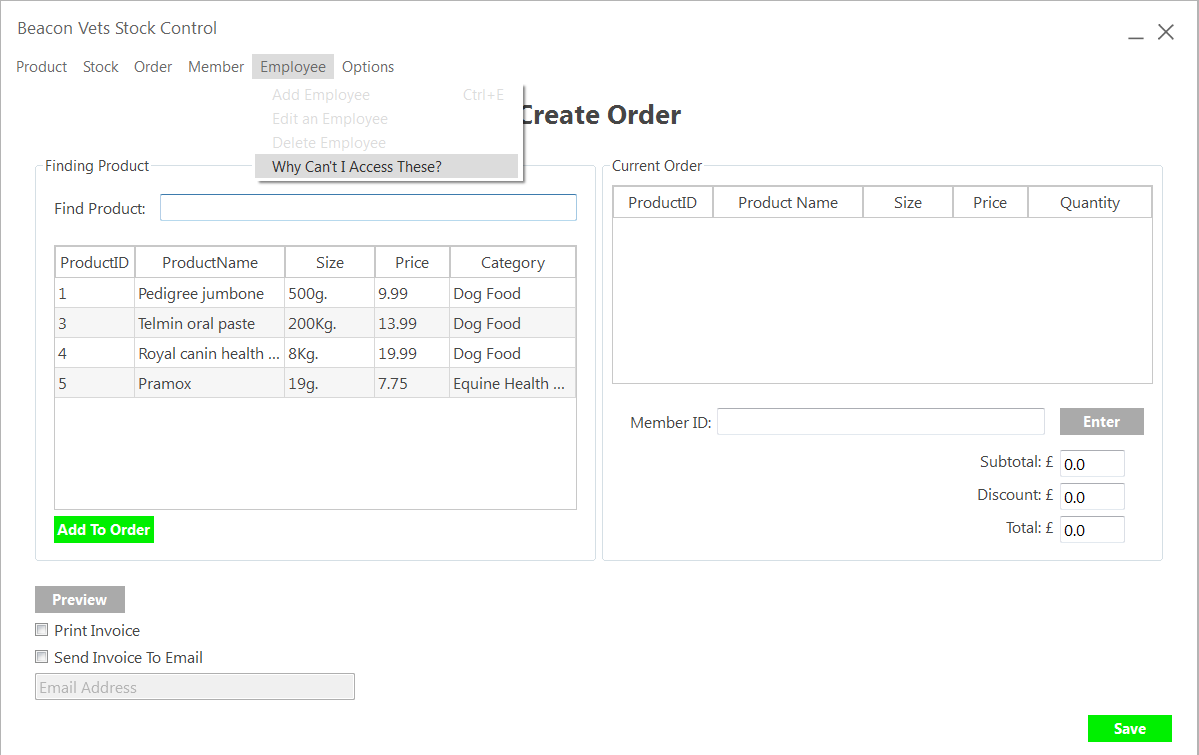
\includegraphics[width=\textwidth]{./110-1.png}
    \caption{Clicking on the why can't i access this option under the Employee menu, if the user is not signed in on the administrators account.} \label{fig:110-1}
\end{figure}

\begin{figure}[H]
    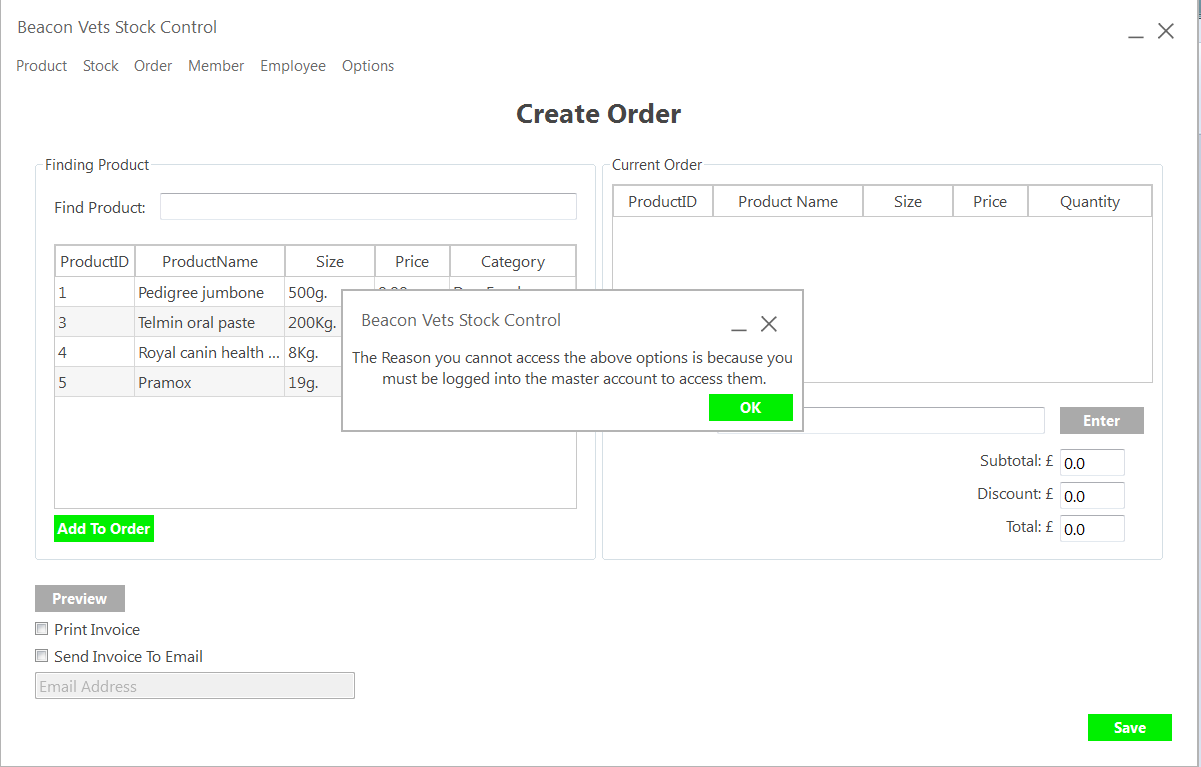
\includegraphics[width=\textwidth]{./110-2.png}
    \caption{A message being displayed when they click on the `Why can't i access this' option under the employee menu.} \label{fig:110-2}
\end{figure}

\begin{figure}[H]
    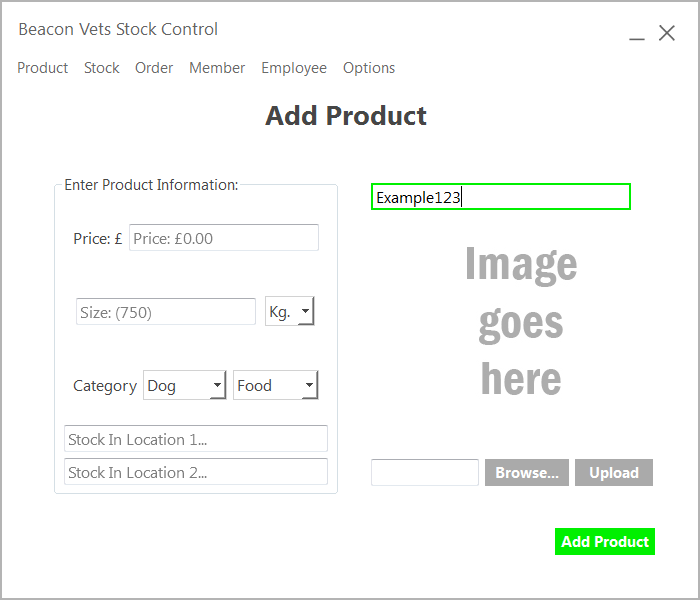
\includegraphics[width=\textwidth]{./201-1.png}
    \caption{Entering a Test into the Product Name field.} \label{fig:201-1}
\end{figure}

\begin{figure}[H]
    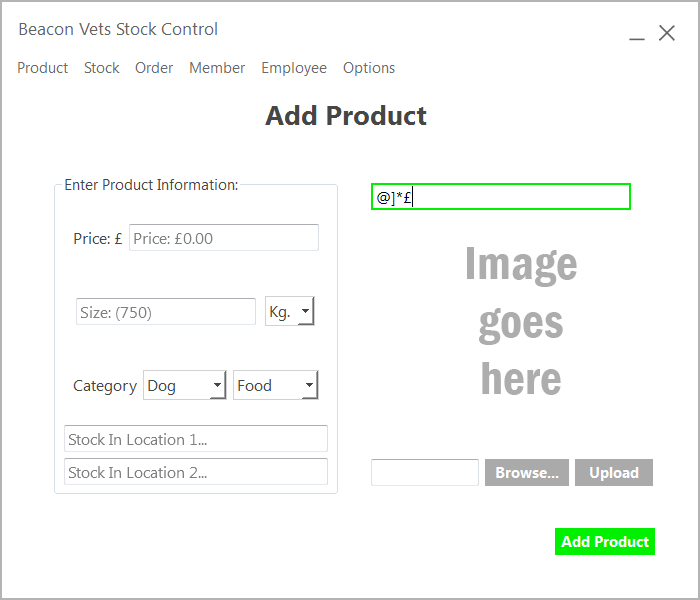
\includegraphics[width=\textwidth]{./201-2.png}
    \caption{Entering Special Characters into the Product Name field.} \label{fig:201-2}
\end{figure}

\begin{figure}[H]
    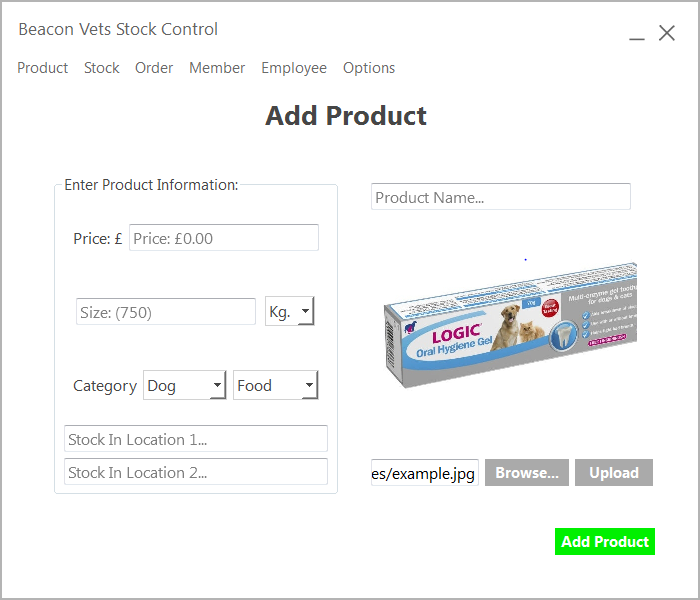
\includegraphics[width=\textwidth]{./202-1.png}
    \caption{using the exmaple.jpg image, and The Image being displayed in the image box.} \label{fig:202-1}
\end{figure}

\begin{figure}[H]
    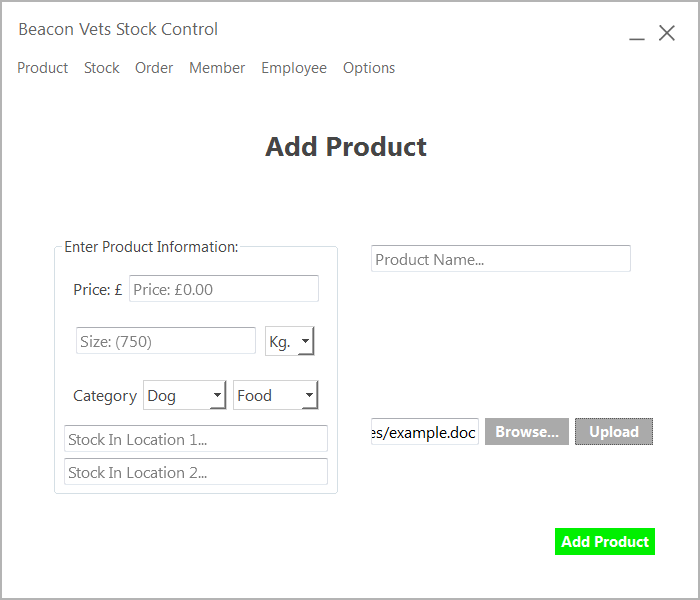
\includegraphics[width=\textwidth]{./202-2.png}
    \caption{Changing the path to an invalid image type.} \label{fig:202-2}
\end{figure}

\begin{figure}[H]
    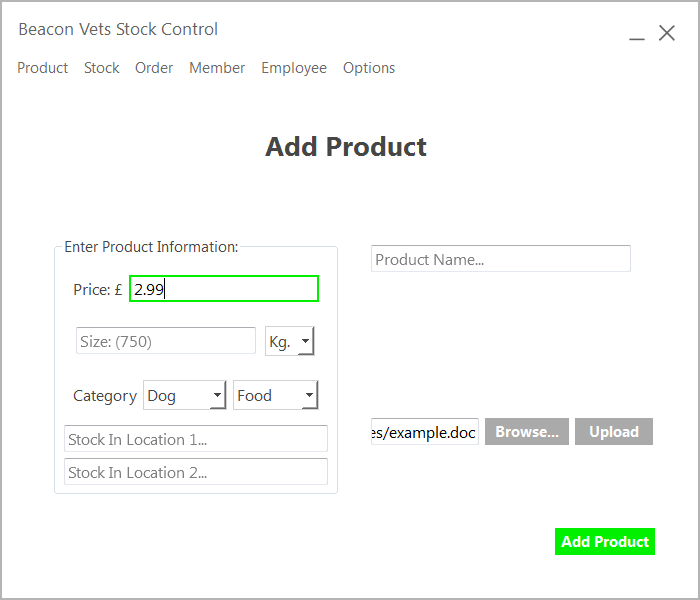
\includegraphics[width=\textwidth]{./203-1.png}
    \caption{Entering Test data into the Price field.} \label{fig:203-1}
\end{figure}

\begin{figure}[H]
    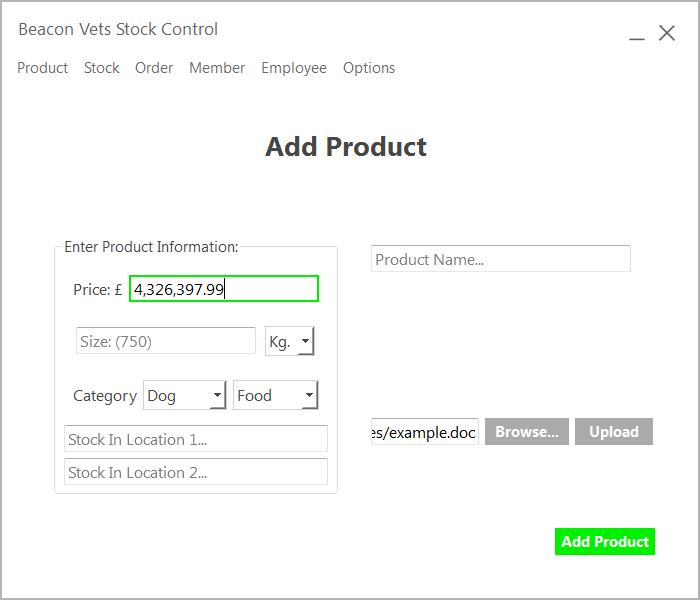
\includegraphics[width=\textwidth]{./203-2.png}
    \caption{Testing the Boundaries of the Price field.} \label{fig:203-2}
\end{figure}

\begin{figure}[H]
    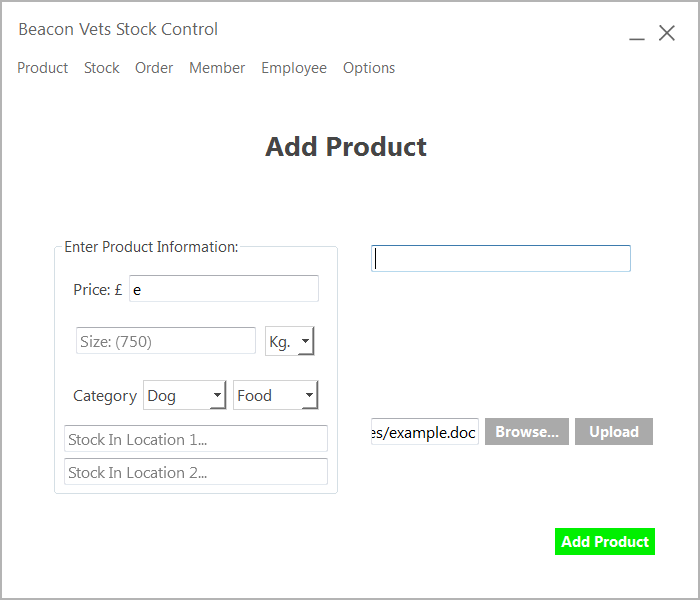
\includegraphics[width=\textwidth]{./203-3.png}
    \caption{Entering example into the price field} \label{fig:203-3}
\end{figure}

\begin{figure}[H]
    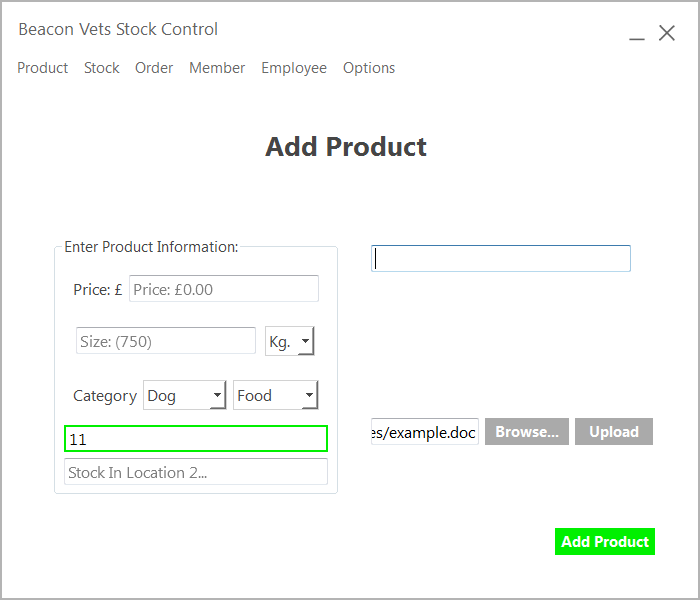
\includegraphics[width=\textwidth]{./204-1.png}
    \caption{Entering Test data into the stock field.} \label{fig:204-1}
\end{figure}

\begin{figure}[H]
    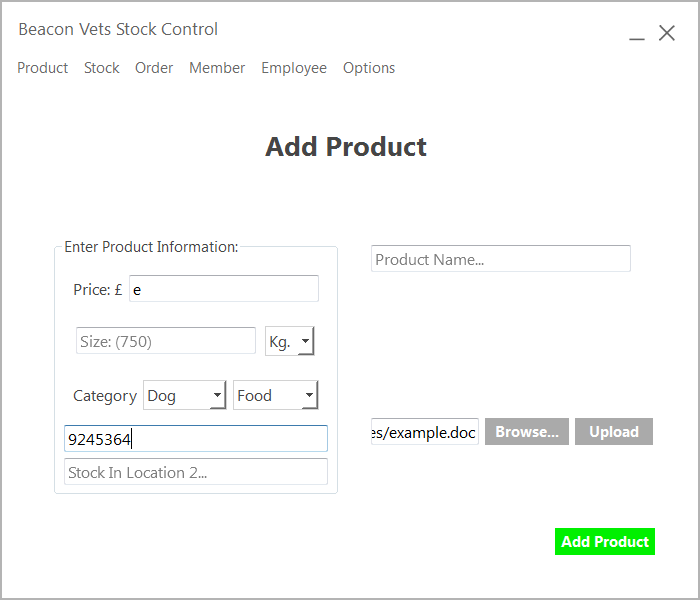
\includegraphics[width=\textwidth]{./204-2.png}
    \caption{Testing the boundaries of the Stock field} \label{fig:204-2}
\end{figure}

\begin{figure}[H]
    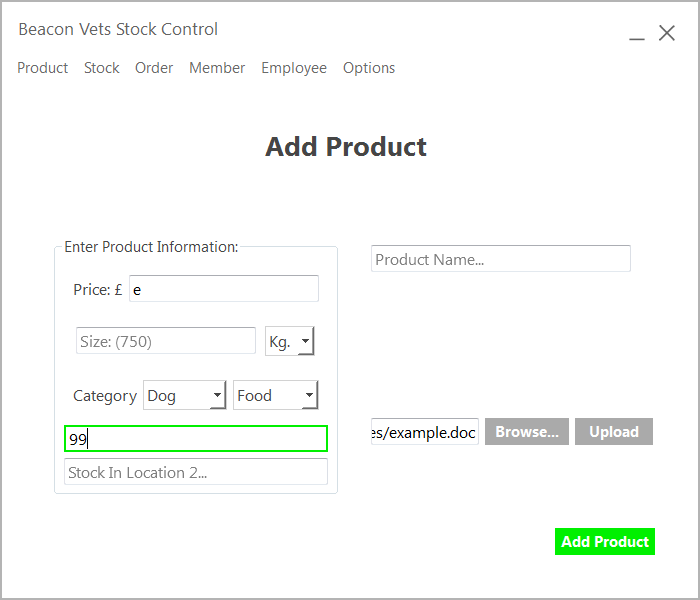
\includegraphics[width=\textwidth]{./204-3.png}
    \caption{Entering 99 in the Stock field} \label{fig:204-3}
\end{figure}

\begin{figure}[H]
    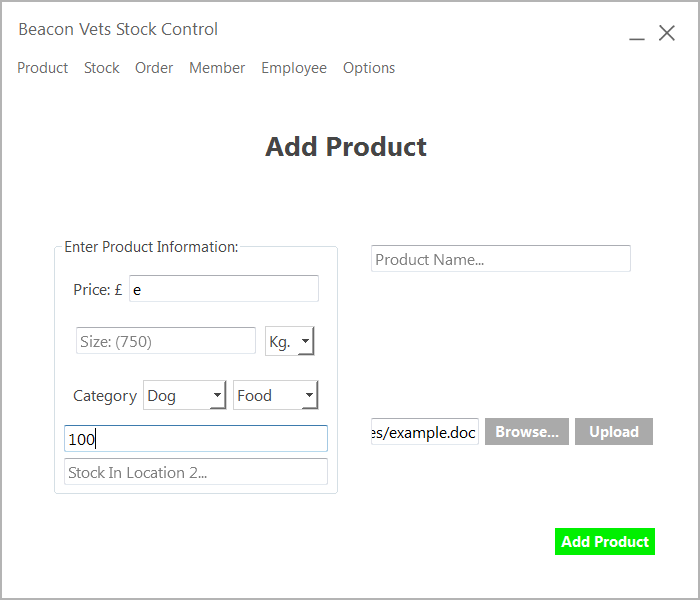
\includegraphics[width=\textwidth]{./204-4.png}
    \caption{Entering 100 into the Stock field.} \label{fig:204-4}
\end{figure}

\begin{figure}[H]
    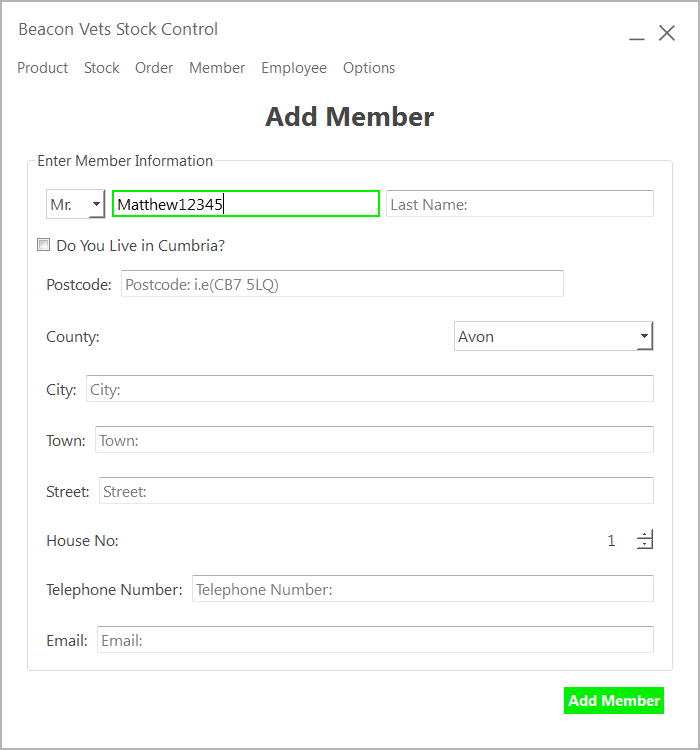
\includegraphics[width=\textwidth]{./205-1.png}
    \caption{Entering Letters and Numbers into the Member First Name field} \label{fig:205-1}
\end{figure}

\begin{figure}[H]
    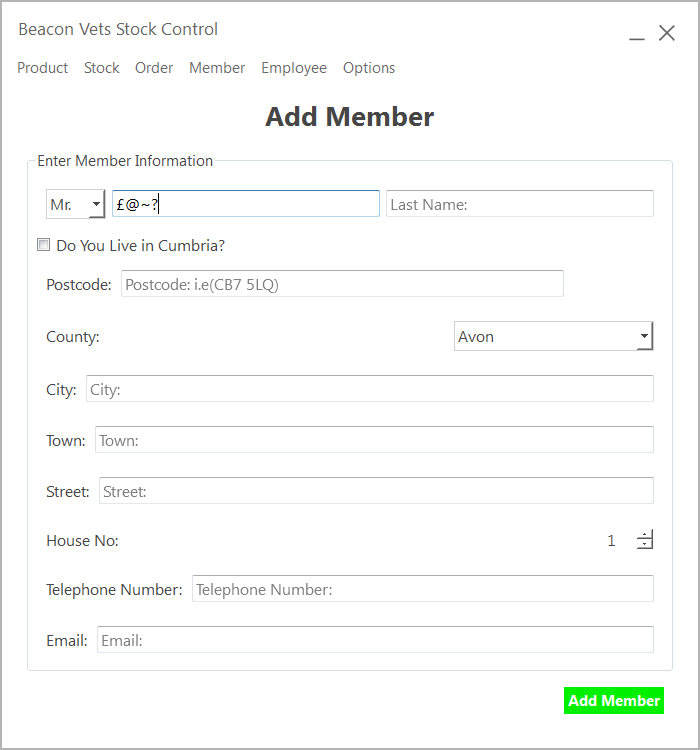
\includegraphics[width=\textwidth]{./205-2.png}
    \caption{Entering special characters into the Members first Name Field} \label{fig:205-2}
\end{figure}

\begin{figure}[H]
    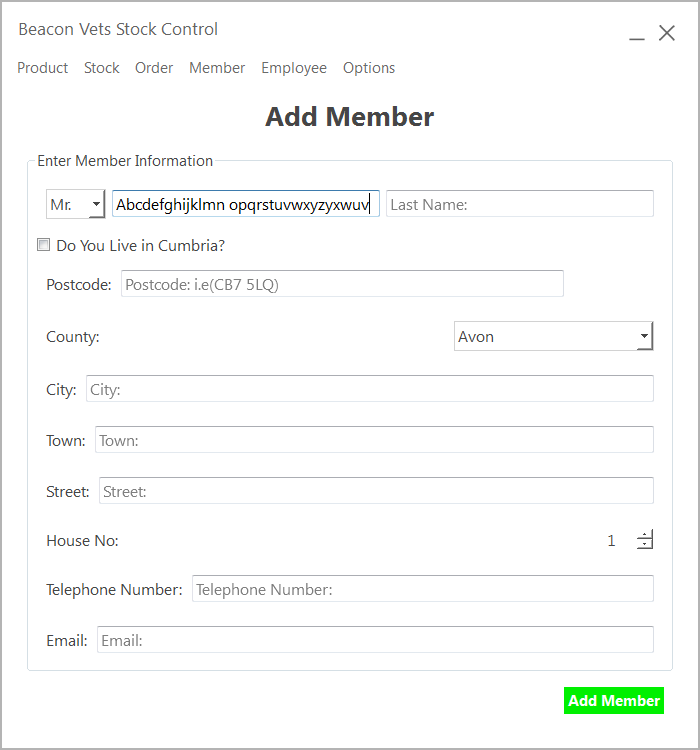
\includegraphics[width=\textwidth]{./205-3.png}
    \caption{Entering a name outside the boundary of the Member First Name} \label{fig:205-3}
\end{figure}

\begin{figure}[H]
    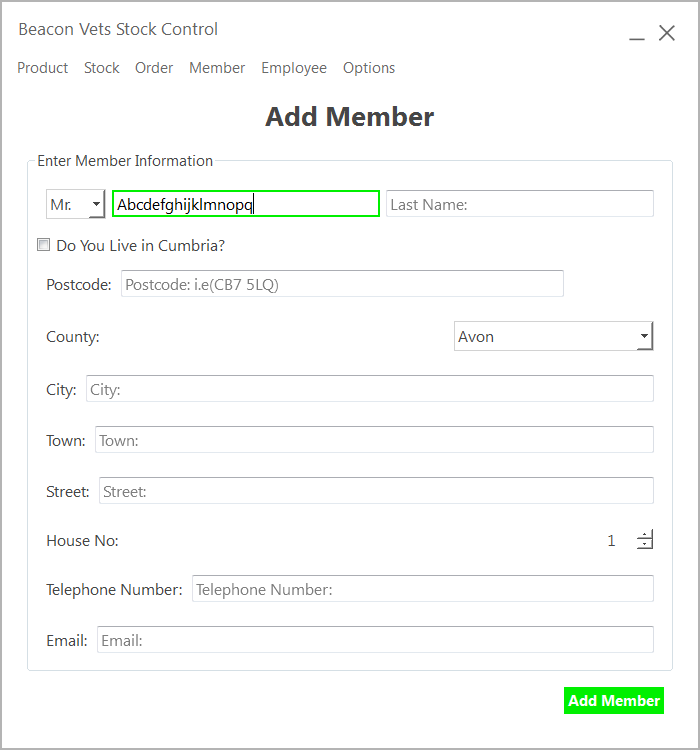
\includegraphics[width=\textwidth]{./205-4.png}
    \caption{Entering a name just inside the boundary of the Member First Name field} \label{fig:205-4}
\end{figure}

\begin{figure}[H]
    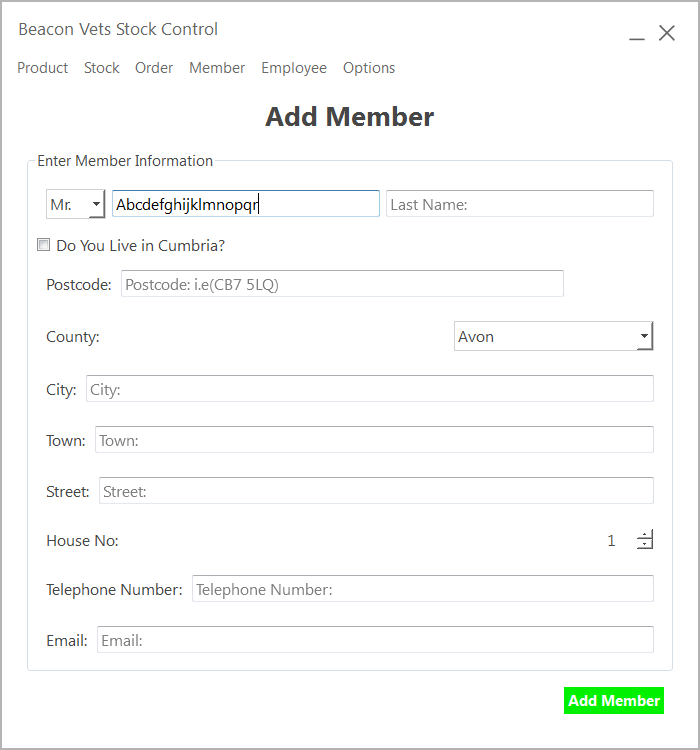
\includegraphics[width=\textwidth]{./205-5.png}
    \caption{Entering a name just outside the boundary of the Member First Name field} \label{fig:205-5}
\end{figure}

\begin{figure}[H]
    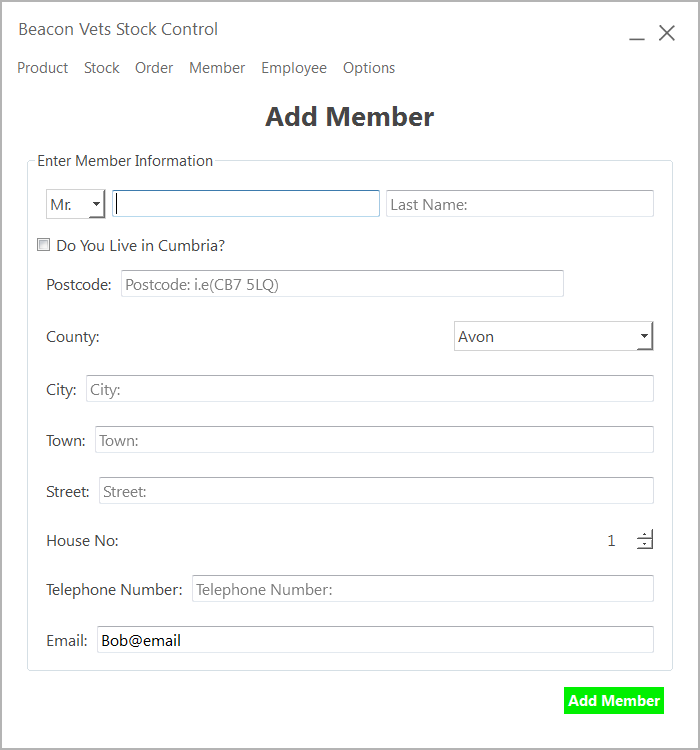
\includegraphics[width=\textwidth]{./206-1.png}
    \caption{Entering test Data into Member Email field.} \label{fig:206-1}
\end{figure}

\begin{figure}[H]
    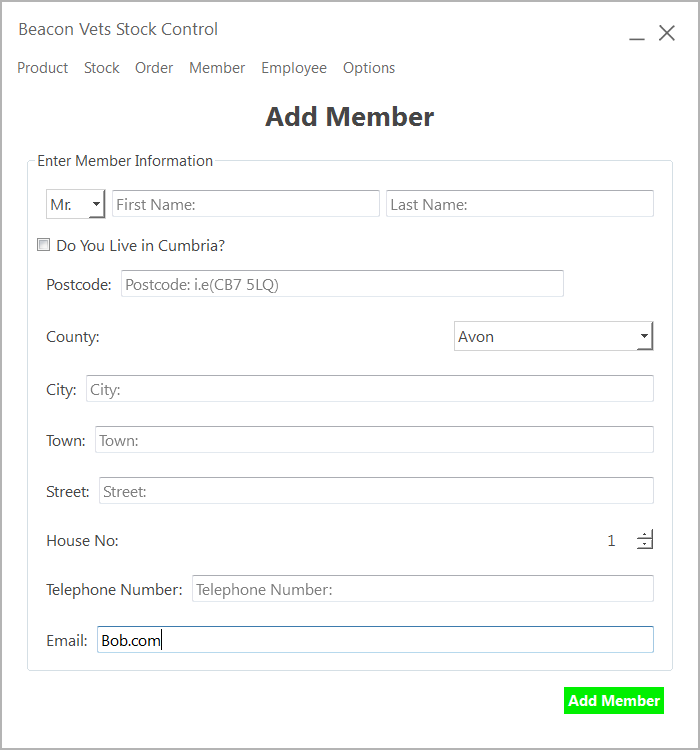
\includegraphics[width=\textwidth]{./206-2.png}
    \caption{Entering an invalid Email address into the Email field} \label{fig:206-2}
\end{figure}

\begin{figure}[H]
    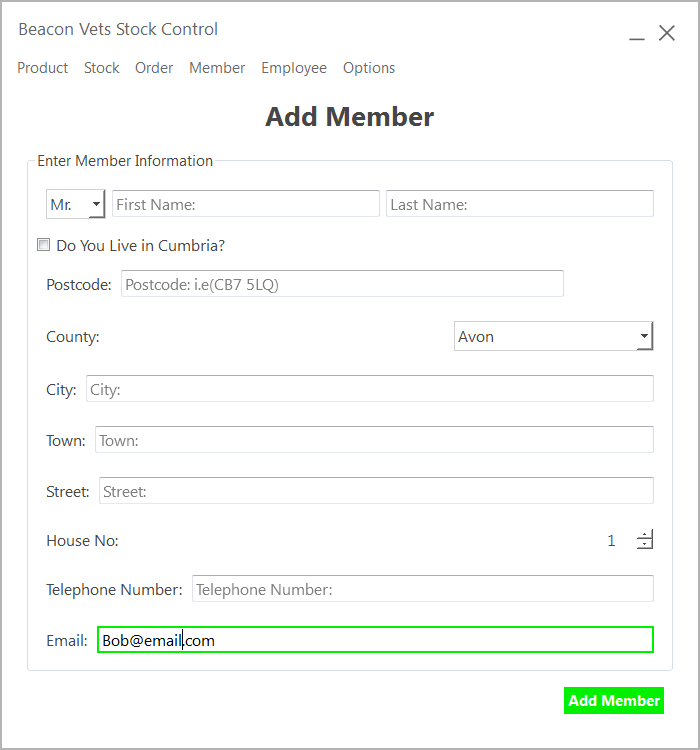
\includegraphics[width=\textwidth]{./206-3.png}
    \caption{Entering a valid Email address into the Email field} \label{fig:206-3}
\end{figure}

\begin{figure}[H]
    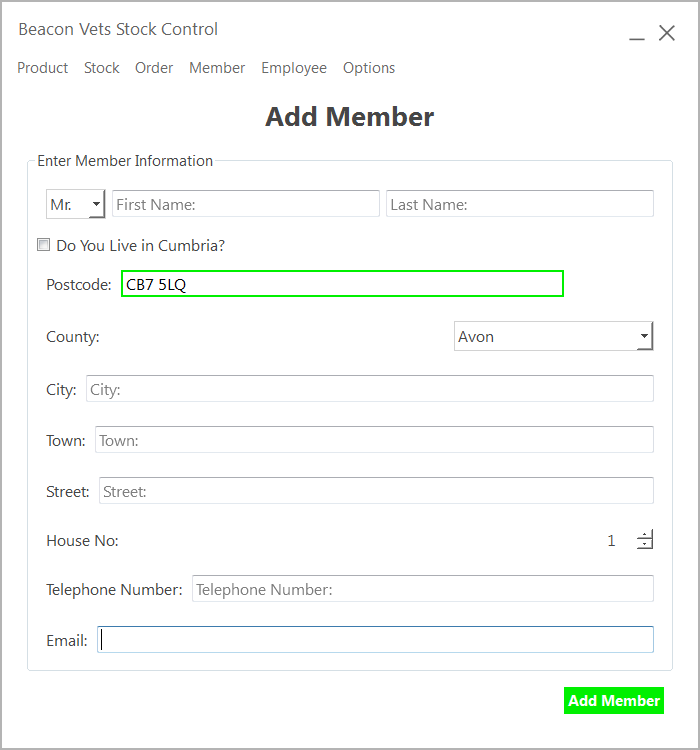
\includegraphics[width=\textwidth]{./207-1.png}
    \caption{Entering test data into the Members Postcode field.} \label{fig:207-1}
\end{figure}

\begin{figure}[H]
    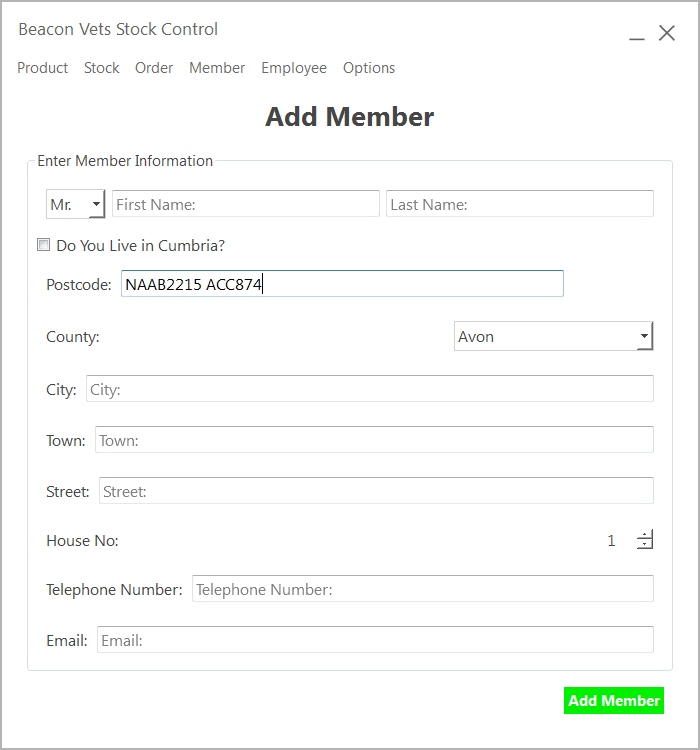
\includegraphics[width=\textwidth]{./207-2.png}
    \caption{Entering an invalid postcode into the Member Postcode field} \label{fig:207-2}
\end{figure}

\begin{figure}[H]
    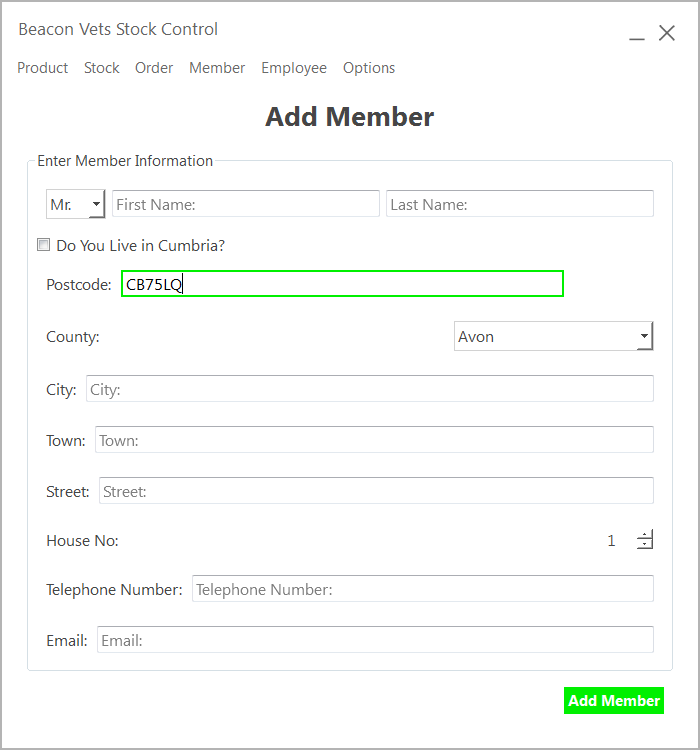
\includegraphics[width=\textwidth]{./207-3.png}
    \caption{Entering a legitimate postcode into the Postcode field} \label{fig:207-3}
\end{figure}

\begin{figure}[H]
    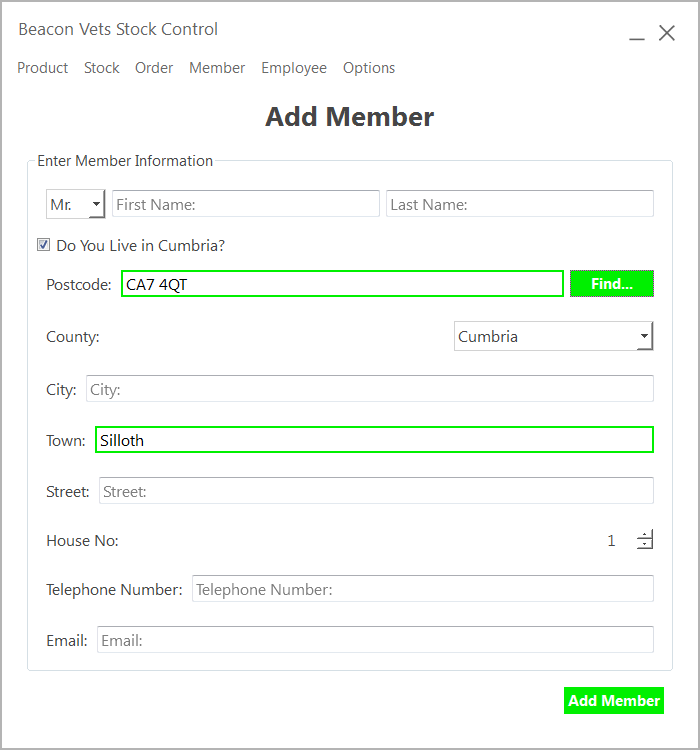
\includegraphics[width=\textwidth]{./208-1.png}
    \caption{Finding a postcode in the CSV file} \label{fig:208-1}
\end{figure}

\begin{figure}[H]
    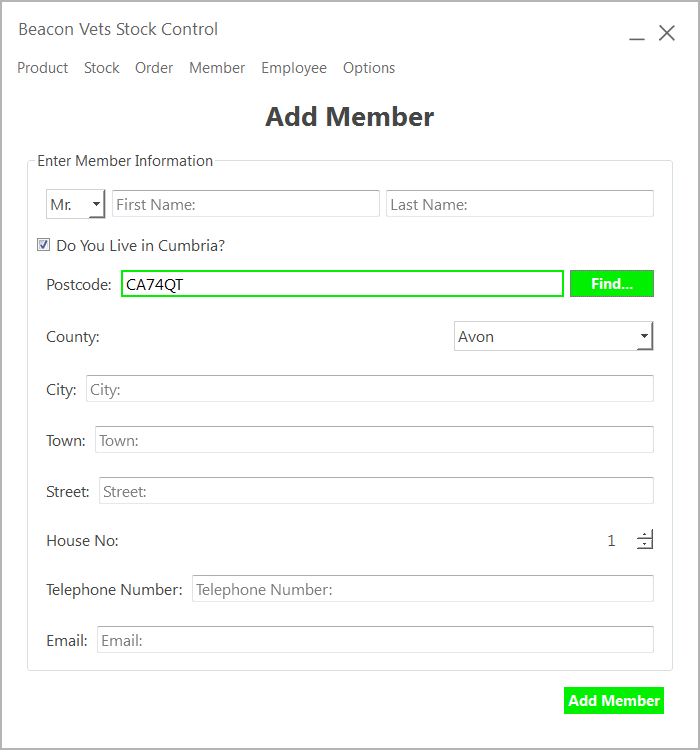
\includegraphics[width=\textwidth]{./208-2.png}
    \caption{Entering Postcode without space and not being found in the CSV file} \label{fig:208-2}
\end{figure}

\begin{figure}[H]
    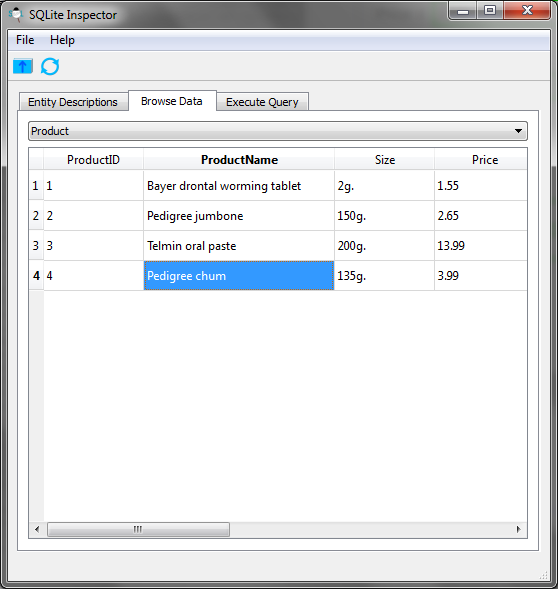
\includegraphics[width=\textwidth]{./301-1.png}
    \caption{The Product Pedigree chum being stored in the Product Name column within the Product Table.} \label{fig:301-1}
\end{figure}

\begin{figure}[H]
    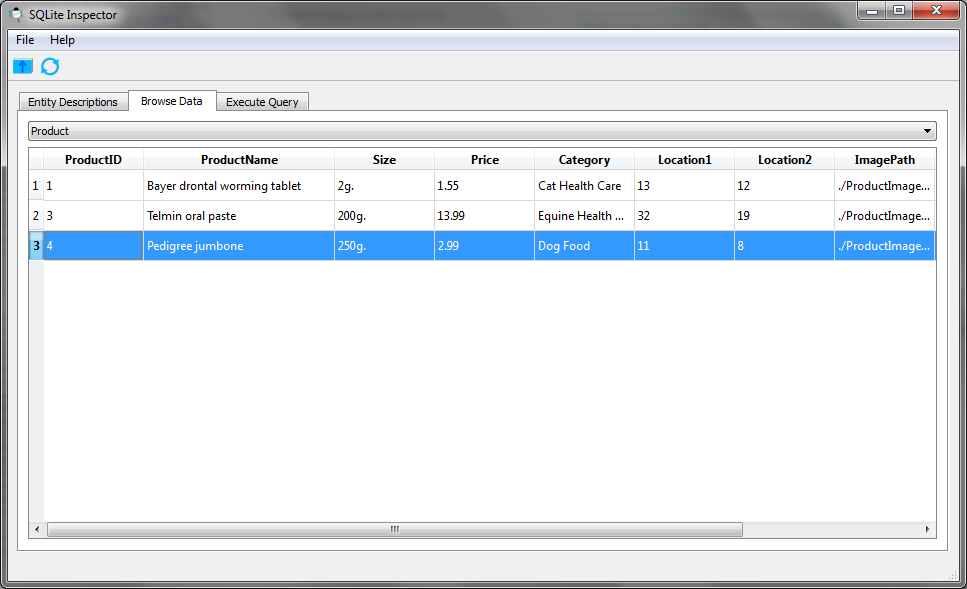
\includegraphics[width=\textwidth]{./303-1.png}
    \caption{All the Product information has been stored in the correct column within the Product table.} \label{fig:303-1}
\end{figure}

\begin{figure}[H]
    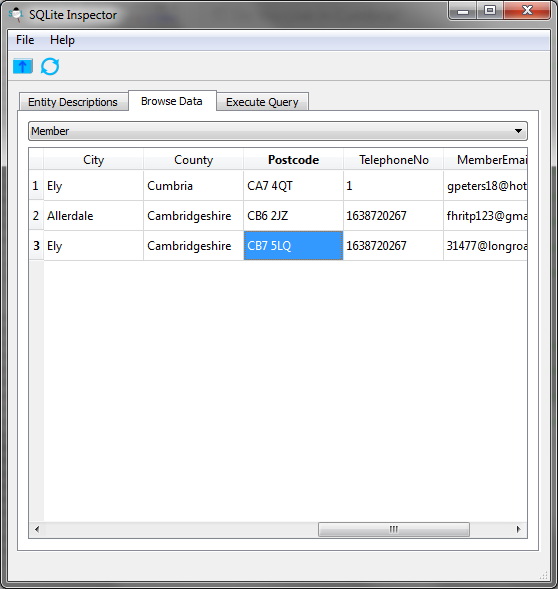
\includegraphics[width=\textwidth]{./304-1.png}
    \caption{The Postcode is stored in the correct column in the Member Table, however, the space ahs not been removed between the two parts of the postcode.} \label{fig:304-1}
\end{figure}

\begin{figure}[H]
    \includegraphics[width=\textwidth]{./305-1.png}
    \caption{All the data associated with the Member has been stored under the correct Column in the Member Table.} \label{fig:305-1}
\end{figure}

\begin{figure}[H]
    \includegraphics[width=\textwidth]{./306-1.png}
    \caption{Logging into an account for the first time using the User-name and the Password: `password' } \label{fig:306-1}
\end{figure}

\begin{figure}[H]
    \includegraphics[width=\textwidth]{./306-2.png}
    \caption{If the user password is `password', they get taken to the Change Your Password interface when logging in. } \label{fig:306-2}
\end{figure}

\begin{figure}[H]
    \includegraphics[width=\textwidth]{./308-1.png}
    \caption{The Stock of the Product in Location1 is currently 20.} \label{fig:308-1}
\end{figure}

\begin{figure}[H]
    \includegraphics[width=\textwidth]{./308-2.png}
    \caption{After Editing the Product in the system, The stock of the Product has now been changed to 15.} \label{fig:308-2}
\end{figure}

\begin{figure}[H]
    \includegraphics[width=\textwidth]{./402-1.png}
    \caption{Showing the Product information before any of the Product Data is changed.} \label{fig:402-1}
\end{figure}

\begin{figure}[H]
    \includegraphics[width=\textwidth]{./402-2.png}
    \caption{Showing the Product information has successfully changed, once updating the Product information within the system} \label{fig:402-2}
\end{figure}

\begin{figure}[H]
    \includegraphics[width=\textwidth]{./403-1.png}
    \caption{Showing the Member information before any changes are made in the system.} \label{fig:403-1}
\end{figure}

\begin{figure}[H]
    \includegraphics[width=\textwidth]{./403-2.png}
    \caption{Showing the Member information has changed after being changed within the system.} \label{fig:403-2}
\end{figure}

\begin{figure}[H]
    \includegraphics[width=\textwidth]{./404-1.png}
    \caption{Showing the Employee information before it is changed in the system.} \label{fig:404-1}
\end{figure}

\begin{figure}[H]
    \includegraphics[width=\textwidth]{./404-2.png}
    \caption{Showing the Employee information has successfully changed after being changed in the system.} \label{fig:404-2}
\end{figure}

\begin{figure}[H]
    \includegraphics[width=\textwidth]{./405-1.png}
    \caption{Showing the Products in the Product table before a Product is removed in the system.} \label{fig:405-1}
\end{figure}

\begin{figure}[H]
    \includegraphics[width=\textwidth]{./405-2.png}
    \caption{Showing that the Product with ProductID of 2 has successfully been removed from the database.} \label{fig:405-2}
\end{figure}

\begin{figure}[H]
    \includegraphics[width=\textwidth]{./406-1.png}
    \caption{Showing The Members in the database before one of them is removed.} \label{fig:406-1}
\end{figure}

\begin{figure}[H]
    \includegraphics[width=\textwidth]{./406-2.png}
    \caption{Showing That the Member with MemberID of 3 has successfully been removed from the database.} \label{fig:406-2}
\end{figure}

\begin{figure}[H]
    \includegraphics[width=\textwidth]{./407-1.png}
    \caption{Showing The Employees in the database before one of them is removed.} \label{fig:407-1}
\end{figure}

\begin{figure}[H]
    \includegraphics[width=\textwidth]{./407-2.png}
    \caption{Showing that The Employee with EmployeeID of 3 has successfully been removed from the system.} \label{fig:407-2}
\end{figure}

\begin{figure}[H]
    \includegraphics[width=\textwidth]{./408-1.png}
    \caption{Showing The Results of When Trying to remove the Admin Employee Account From the System (EmployeeID of 1)} \label{fig:408-1}
\end{figure}

\begin{figure}[H]
    \includegraphics[width=\textwidth]{./501-1.png}
    \caption{Entering The Email and password into to the Email Account field at the preferences interface.} \label{fig:501-1}
\end{figure}

\begin{figure}[H]
    \includegraphics[width=\textwidth]{./501-1.png}
    \caption{Entering The Email and password into to the Email Account field at the preferences interface.} \label{fig:501-1}
\end{figure}

\begin{figure}[H]
    \includegraphics[width=\textwidth]{./501-2.png}
    \caption{Creating an Order, Entering the MemberID of 1 , then choosing to send the invoice by email.} \label{fig:501-2}
\end{figure}

\begin{figure}[H]
    \includegraphics[width=\textwidth]{./501-3.png}
    \caption{Showing that the Member received the email, proving the email address and password are valid.} \label{fig:501-3}
\end{figure}

\begin{figure}[H]
    \includegraphics[width=\textwidth]{./502-1.png}
    \caption{ The user clicking on the change password option under the Options Menu. } \label{fig:502-1}
\end{figure}

\begin{figure}[H]
    \includegraphics[width=\textwidth]{./502-2.png}
    \caption{The Change Password Interface being displayed.} \label{fig:502-2}
\end{figure}

\begin{figure}[H]
    \includegraphics[width=\textwidth]{./504-1.png}
    \caption{Showing the Subjects of the three types of email that are sent.} \label{fig:504-1}
\end{figure}

\begin{figure}[H]
    \includegraphics[width=\textwidth]{./601-1.png}
    \caption{Pressing the ESC button when logged in, opens the Log off confirmation window.} \label{fig:601-1}
\end{figure}

\begin{figure}[H]
    \includegraphics[width=\textwidth]{./603-1.png}
    \caption{When CTRL and F are pressed when logged in, the search window is displayed.} \label{fig:603-1}
\end{figure}

\begin{figure}[H]
    \includegraphics[width=\textwidth]{./604-1.png}
    \caption{Pressing CTRL and S whilst on the Add Product interface opens the Add Product confirmation window.} \label{fig:604-1}
\end{figure}

\begin{figure}[H]
    \includegraphics[width=\textwidth]{./604-2.png}
    \caption{Pressing CTRL and S whilst on the Edit Product interface opens the Edit Product confirmation window.} \label{fig:604-2}
\end{figure}

\begin{figure}[H]
    \includegraphics[width=\textwidth]{./604-3.png}
    \caption{Pressing CTRL and S whilst on the Delete Product interface opens the Delete Product confirmation window.} \label{fig:604-3}
\end{figure}

\begin{figure}[H]
    \includegraphics[width=\textwidth]{./604-4.png}
    \caption{Pressing CTRL and S whilst on the Add Member interface opens the Add Member confirmation window.} \label{fig:604-4}
\end{figure}

\begin{figure}[H]
    \includegraphics[width=\textwidth]{./604-5.png}
    \caption{Pressing CTRL and S whilst on the Edit Member interface opens the Edit Member confirmation window.} \label{fig:604-5}
\end{figure}

\begin{figure}[H]
    \includegraphics[width=\textwidth]{./604-6.png}
    \caption{Pressing CTRL and S whilst on the Delete Member interface opens the Delete Member confirmation window.} \label{fig:604-6}
\end{figure}

\begin{figure}[H]
    \includegraphics[width=\textwidth]{./604-7.png}
    \caption{Pressing CTRL and S whilst on the Add Employee interface opens the Add Employee confirmation window.} \label{fig:604-7}
\end{figure}

\begin{figure}[H]
    \includegraphics[width=\textwidth]{./604-8.png}
    \caption{Pressing CTRL and S whilst on the Edit Employee interface opens the Edit Employee confirmation window.} \label{fig:604-8}
\end{figure}

\begin{figure}[H]
    \includegraphics[width=\textwidth]{./604-9.png}
    \caption{Pressing CTRL and S whilst on the Delete Employee interface opens the Delete Employee confirmation window.} \label{fig:604-9}
\end{figure}

\begin{figure}[H]
    \includegraphics[width=\textwidth]{./605-1.png}
    \caption{Pressing the Enter button on the keyboard opens up the confirmation window will open another window saying the Product/Employee/Member has successfully been Added/Edited/Deleted} \label{fig:605-1}
\end{figure}

\begin{figure}[H]
    \includegraphics[width=\textwidth]{./606-1.png}
    \caption{Right clicking on a product in the search window opens the Product Menu.} \label{fig:606-1}
\end{figure}

\begin{figure}[H]
    \includegraphics[width=\textwidth]{./606-2.png}
    \caption{Right clicking on a Member in the search window opens the Member Menu.} \label{fig:606-2}
\end{figure}

\begin{figure}[H]
    \includegraphics[width=\textwidth]{./606-3.png}
    \caption{Right clicking on an Employee in the search window opens the Employee Menu.} \label{fig:606-3}
\end{figure}
